\documentclass[12pt,a4paper]{scrartcl}
\usepackage[T1]{fontenc}
\usepackage[utf8x]{inputenc}
\usepackage{lscape}
\usepackage[ngerman]{babel}
\usepackage{fancyhdr}
\usepackage{amsmath}
\usepackage{amsthm}
\usepackage{amsfonts}
\usepackage{amssymb}
\usepackage{marvosym}
\usepackage{bbm}
\usepackage{mathtools}
\usepackage{array}
\usepackage{paralist}
\usepackage{tabularx}
\usepackage{caption}
\usepackage{listings}
\usepackage{multirow}
\usepackage[ruled]{algorithm}
%\usepackage{algorithmicx}
\usepackage{algpseudocode}
\usepackage{hyperref}
\usepackage{textcomp}
%\usepackage{ulsy}
\usepackage{array}
%Bäume, Automaten:
%\usepackage{qtree}
\usepackage{pgf}
\usepackage{tikz}
\usetikzlibrary{arrows,automata}
\usepackage{gensymb}
\usepackage{siunitx}
\usepackage{pgfplots}
%Seitenlayout
\usepackage{fancyhdr}
\usepackage{lastpage}
\pagestyle{fancy}
\renewcommand{\headrulewidth}{1pt}
\renewcommand{\footrulewidth}{0.4pt}
\fancyheadoffset{30pt}
\setlength{\headheight}{41pt}
\newcommand{\N}{\ensuremath{\mathbb{N}}}
\newcommand{\Z}{\ensuremath{\mathbb{Z}}}
\newcommand{\Q}{\ensuremath{\mathbb{Q}}}
\newcommand{\R}{\ensuremath{\mathbb{R}}}
\newcommand{\C}{\ensuremath{\mathbb{C}}}
\newcommand{\ggT}{\text{ggT}}
\newcommand{\abs}[1]{\ensuremath{ | #1 |}}
\newcommand{\norm}[1]{\ensuremath{ \lVert #1 \rVert}}
\newcommand{\qq}[1]{\glqq #1\grqq}
\newcommand{\todo}[1]{{\color{red}\textbf{TODO: #1}}}
\renewcommand{\matrix}[1]{\begin{pmatrix}#1\end{pmatrix}}
%Schicke Vektoren mit \vec{}
\newcount\colveccount
\newcommand*\colvec[1]{
	\global\colveccount#1
	\begin{pmatrix}
		\colvecnext
	}
	\def\colvecnext#1{
		#1
		\global\advance\colveccount-1
		\ifnum\colveccount>0
		\\
		\expandafter\colvecnext
		\else
	\end{pmatrix}
	\fi
}



\renewcommand{\labelenumi}{(\alph{enumi})}
%\renewcommand{\thesubsection}{Exercise \arabic{subsection}}
\lhead{Marius Hobbhahn\\Marc Tomasek}
\chead{{\Large Artificial Intelligence}\\ {\Large Übungsblatt 2}}
\rhead{\today}
\cfoot{{Seite \thepage} von \pageref*{LastPage}}
\begin{document}
	
\section{}
	I didn't see that we need to start at $x_0$ but the principle is exactly the same. I hope you are able to acknowledge the understanding of the procedure. I am unfortunatly unable to rescan the pictures because the library is closed. 
	\subsection*{a)}
		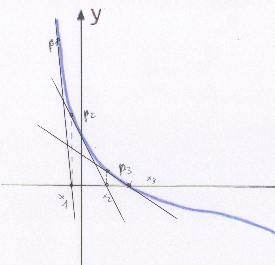
\includegraphics[width = 0.7\textwidth]{figure_1a.png} \\
		In this case we always take the slope of the function in a given point $p$ and check where a linear function with this slope meets the x-Axis. From the same x-Coordinate we again take the slope and repeat the procedure until the point at which we meet the x-Axis is also the coordinate we would jump to, meaning y = 0.
	\subsection*{b)}
		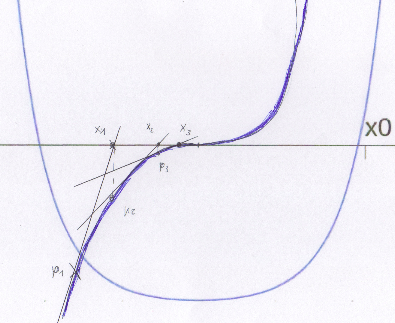
\includegraphics[width = 0.7\textwidth]{figure_1b.png} \\
		For the minimum we want to use the same procedure like in a) though not on the function itself but on the first derivative. The given function looks like one of degree 4, the first derivative therefore is one of degree 3. On this we then apply the same idea as in a). This can be seen in the first graphic. \\
		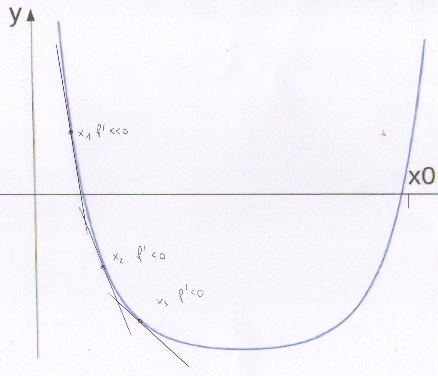
\includegraphics[width = 0.7\textwidth]{figure_1b_2.png} \\
		From the assignment text it is unclear whether the function is given, or allowed to be assumed. A second version therefore is to just derive locally and go right if the value is negative and left if the derivative is positive. The distance that we go further in the given direction is proportional to the size of the result, i.e. very negative first derivatives lead to big jumps to the right and small negative results to small jumps. 
	\subsection*{c)}
	\begin{figure}[!h]
		\centering
		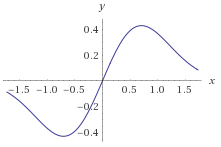
\includegraphics[width = \textwidth]{AI1c.png}
		\caption{function for 1c)}
	\end{figure}
	The function $f(x) = x \cdot e^{-x^2}$ never converges to the root at 0 if you choose starting points too far off - that means left of the negative peak or right of the positive peak, we will be thrown of to (negative) infinity, never converging to 0.
	\subsection*{d)}
	$$f(x_1,x_2) = x_1^2 - 2x_1^3 + 2 \exp(x_1) - \exp(-x_2^2) - 3$$
	Gradient/Jacobian: $$(2x_1 - 6x_1^2 + 2e^{x_1}, 2e^{-x_2^2})$$
	Hessian of f:\\
	$$\begin{pmatrix}
		\frac{\delta^2 f}{\delta x_1^2} & \frac{\delta^2 f}{\delta x_1x_2} \\
		\frac{\delta^2 f}{\delta x_2x_1} & \frac{\delta^2 f}{\delta x_2^2} \\
	\end{pmatrix} 
	= \begin{pmatrix}
		2 - 12x_1 + 2e^{x_1} & 0 \\
		0 & e^{(-x^2)} \cdot (2 - 4 x^2)
	\end{pmatrix}
	$$
	Inverted Hessian of f: \\
	$$\begin{pmatrix}
		\frac{1}{2 - 12x_1 + 2e^{x_1}} & 0 \\
		0 & \frac{1}{e^{(-x_2^2)} \cdot (2 - 4 x_2^2)}
	\end{pmatrix}$$
	Every update step is now calculated as $x \leftarrow x - H_f^{-1} (x) \cdot \nabla f(x)$\\
	That means our first step is: \\
	\begin{align*}
		x_1, x_2 &= (-1,0.1) - \begin{pmatrix}
		\frac{1}{2 - 12\cdot -1 + 2e^{-1}} & 0 \\
		0 & \frac{1}{e^{(-0.1^2)} \cdot (2 - 4 \cdot 0.1^2)} 
		\end{pmatrix} 
		\cdot (2 \cdot -1 - 6 \cdot -1^2 + 2e^{-1}, 2e^{-0.1^2}) \\
		&= (-1,0.1) - (0.32, 1.02) \\
		&= (-1.32, -0.92)
	\end{align*}
	And the second step: \\
	\begin{align*}
		x_1, x_2 &= (-1.32, -0.92) - \begin{pmatrix}
			\frac{1}{2 - 12\cdot -1.32 + 2e^{-1.32}} & 0 \\
			0 & \frac{1}{e^{(-0.92^2)} \cdot (2 - 4 \cdot 0.92^2)}
		\end{pmatrix} \cdot 
		(2 \cdot -1.32 - 6 \cdot -1.32^2 + 2e^{-1.32}, 2e^{-0.92^2}) \\
		&= (-1.32,-0.92) - (0.45, -1.44)\\
		&= (-1.77, 0.52)
	\end{align*}
\section{}
	\subsection*{a)}
	\begin{center}
		\begin{tikzpicture}[scale=0.2]
		\tikzstyle{every node}+=[inner sep=0pt]
		\draw [black] (38.2,-23.9) circle (3);
		\draw (38.2,-23.9) node {$abcd$};
		\draw [black] (53.6,-24.2) circle (3);
		\draw (53.6,-24.2) node {$bd$};
		\draw [black] (63.8,-31.8) circle (3);
		\draw (63.8,-31.8) node {$cd$};
		\draw [black] (76.3,-36.8) circle (3);
		\draw (76.3,-36.8) node {$d$};
		\draw [black] (63.8,-47.5) circle (3);
		\draw (63.8,-47.5) node {$c$};
		\draw [black] (38.8,-37.7) circle (3);
		\draw (38.8,-37.7) node {$acd$};
		\draw [black] (38.8,-9.2) circle (3);
		\draw (38.8,-9.2) node {$abd$};
		\draw [black] (22.1,-23.9) circle (3);
		\draw (22.1,-23.9) node {$ac$};
		\draw [black] (5.9,-33.1) circle (3);
		\draw (5.9,-33.1) node {$a$};
		\draw [black] (17.2,-35) circle (3);
		\draw (17.2,-35) node {$ab$};
		\draw [black] (17.8,-46.8) circle (3);
		\draw (17.8,-46.8) node {$b$};
		\draw [black] (51.44,-26.264) arc (-55.31598:-126.91604:9.542);
		\fill [black] (51.44,-26.26) -- (50.5,-26.31) -- (51.07,-27.13);
		\draw (45.81,-28.48) node [below] {$R$};
		\draw [black] (24.643,-22.322) arc (115.17757:64.82243:12.944);
		\fill [black] (24.64,-22.32) -- (25.58,-22.43) -- (25.15,-21.53);
		\draw (30.15,-20.59) node [above] {$L$};
		\draw [black] (38.32,-20.9) -- (38.68,-12.2);
		\fill [black] (38.68,-12.2) -- (38.15,-12.98) -- (39.14,-13.02);
		\draw (39.06,-16.56) node [right] {$U$};
		\draw [black] (38.33,-26.9) -- (38.67,-34.7);
		\fill [black] (38.67,-34.7) -- (39.13,-33.88) -- (38.14,-33.93);
		\draw (37.94,-30.82) node [left] {$D$};
		\draw [black] (40.796,-11.436) arc (37.40311:-37.40311:19.779);
		\fill [black] (40.8,-35.46) -- (41.68,-35.13) -- (40.88,-34.52);
		\draw (45.36,-23.45) node [right] {$D$};
		\draw [black] (36.902,-35.38) arc (-144.8656:-215.1344:20.73);
		\fill [black] (36.9,-11.52) -- (36.03,-11.89) -- (36.85,-12.46);
		\draw (32.63,-23.45) node [left] {$U$};
		\draw [black] (41.619,-10.219) arc (66.10503:23.12591:21.376);
		\fill [black] (52.62,-21.37) -- (52.76,-20.44) -- (51.84,-20.83);
		\draw (48.7,-13.28) node [right] {$R$};
		\draw [black] (52.461,-26.972) arc (-26.56636:-68.69387:20.328);
		\fill [black] (52.46,-26.97) -- (51.66,-27.46) -- (52.55,-27.91);
		\draw (49.24,-33.39) node [below] {$R$};
		\draw [black] (22.794,-20.985) arc (161.61011:101.10091:17.222);
		\fill [black] (22.79,-20.99) -- (23.52,-20.38) -- (22.57,-20.07);
		\draw (26.6,-13) node [above] {$L$};
		\draw [black] (36.162,-36.272) arc (-120.20467:-138.93239:48.487);
		\fill [black] (24,-26.22) -- (24.15,-27.15) -- (24.9,-26.5);
		\draw (28.51,-32.24) node [below] {$L$};
		\draw [black] (21.528,-20.959) arc (185.77415:-6.86546:16.45);
		\fill [black] (54.23,-21.27) -- (54.82,-20.54) -- (53.83,-20.42);
		\draw (38.05,-2.34) node [above] {$R$};
		\draw [black] (53.8,-27.189) arc (-1.55719:-179.53413:15.981);
		\fill [black] (21.84,-26.88) -- (21.35,-27.69) -- (22.35,-27.68);
		\draw (37.67,-43.25) node [below] {$L$};
		\draw [black] (36.541,-39.656) arc (-21.37913:-309.37913:2.25);
		\draw (31.5,-39.89) node [left] {$D$};
		\fill [black] (35.87,-37.1) -- (35.31,-36.34) -- (34.95,-37.27);
		\draw [black] (41.099,-7.29) arc (157.45076:-130.54924:2.25);
		\draw (46.12,-7.2) node [right] {$U$};
		\fill [black] (41.71,-9.86) -- (42.26,-10.63) -- (42.64,-9.71);
		\draw [black] (74.977,-34.12) arc (234:-54:2.25);
		\draw (76.3,-29.55) node [above] {$R,U,D$};
		\fill [black] (77.62,-34.12) -- (78.5,-33.77) -- (77.69,-33.18);
		\draw [black] (4.577,-30.42) arc (234:-54:2.25);
		\draw (5.9,-25.85) node [above] {$L,U,D$};
		\fill [black] (7.22,-30.42) -- (8.1,-30.07) -- (7.29,-29.48);
		\draw [black] (15.439,-44.95) arc (-130.23264:-147.81134:40.107);
		\fill [black] (15.44,-44.95) -- (15.15,-44.05) -- (14.51,-44.81);
		\draw (10.52,-42.08) node [left] {$R$};
		\draw [black] (14.863,-47.351) arc (-88.19371:-189.85027:9.755);
		\fill [black] (4.94,-35.93) -- (4.31,-36.63) -- (5.3,-36.8);
		\draw (6.65,-45.45) node [left] {$L$};
		\draw [black] (60.86,-48.095) arc (-79.40749:-102.33616:100.986);
		\fill [black] (20.72,-47.48) -- (21.4,-48.14) -- (21.61,-47.17);
		\draw (40.75,-50.32) node [below] {$U$};
		\draw [black] (61.254,-49.086) arc (-60.22173:-121.52192:40.176);
		\fill [black] (61.25,-49.09) -- (60.31,-49.05) -- (60.81,-49.92);
		\draw (40.68,-54.91) node [below] {$D$};
		\draw [black] (74.79,-39.389) arc (-34.38928:-64.48367:20.785);
		\fill [black] (74.79,-39.39) -- (73.93,-39.77) -- (74.75,-40.33);
		\draw (72.41,-43.93) node [below] {$R$};
		\draw [black] (77.066,-39.685) arc (4.82032:-103.69327:8.543);
		\fill [black] (66.53,-48.7) -- (67.19,-49.38) -- (67.43,-48.41);
		\draw (75.27,-47.38) node [below] {$L$};
		\draw [black] (18.51,-49.703) arc (41.47119:-246.52881:2.25);
		\draw (14.87,-54.08) node [below] {$U,R$};
		\fill [black] (15.93,-49.13) -- (15,-49.28) -- (15.66,-50.03);
		\draw [black] (65.524,-49.941) arc (62.97263:-225.02737:2.25);
		\draw (65.74,-54.87) node [below] {$D,L$};
		\fill [black] (62.91,-50.35) -- (62.1,-50.84) -- (62.99,-51.29);
		\draw [black] (17.35,-38) -- (17.65,-43.8);
		\fill [black] (17.65,-43.8) -- (18.11,-42.98) -- (17.11,-43.03);
		\draw (16.92,-40.92) node [left] {$R$};
		\draw [black] (14.24,-34.5) -- (8.86,-33.6);
		\fill [black] (8.86,-33.6) -- (9.56,-34.22) -- (9.73,-33.24);
		\draw (12.06,-33.44) node [above] {$L$};
		\draw [black] (15.589,-32.501) arc (-160.50601:-247.13129:6.459);
		\fill [black] (19.17,-24.39) -- (18.24,-24.24) -- (18.63,-25.17);
		\draw (15.04,-26.75) node [left] {$D$};
		\draw [black] (20.89,-26.64) -- (18.41,-32.26);
		\fill [black] (18.41,-32.26) -- (19.19,-31.73) -- (18.28,-31.32);
		\draw (18.92,-28.47) node [left] {$U$};
		\draw [black] (20.105,-35.7) arc (104.19443:-183.80557:2.25);
		\draw (22.94,-40.76) node [right] {$U$};
		\fill [black] (18.41,-37.73) -- (18.12,-38.63) -- (19.09,-38.38);
		\draw [black] (73.378,-36.126) arc (-105.49929:-118.10353:34.324);
		\fill [black] (73.38,-36.13) -- (72.74,-35.43) -- (72.47,-36.39);
		\draw (68.61,-35.44) node [below] {$R$};
		\draw [black] (62.59,-44.759) arc (-161.51601:-198.48399:16.116);
		\fill [black] (62.59,-44.76) -- (62.81,-43.84) -- (61.86,-44.16);
		\draw (61.26,-39.65) node [left] {$L$};
		\draw [black] (63.727,-28.813) arc (209.12526:-78.87474:2.25);
		\draw (67.92,-25.17) node [above] {$D$};
		\fill [black] (66.13,-29.93) -- (67.07,-29.97) -- (66.58,-29.1);
		\draw [black] (56.366,-25.355) arc (63.10203:43.51852:20.299);
		\fill [black] (61.9,-29.48) -- (61.71,-28.56) -- (60.99,-29.24);
		\draw (60.61,-26.68) node [above] {$D$};
		\draw [black] (61.054,-30.597) arc (-117.60154:-135.7779:21.776);
		\fill [black] (55.54,-26.49) -- (55.74,-27.41) -- (56.45,-26.71);
		\draw (56.78,-29.26) node [below] {$U$};
		\draw [black] (55.512,-21.903) arc (167.96249:-120.03751:2.25);
		\draw (60.49,-20.47) node [right] {$R,U$};
		\fill [black] (56.59,-24.32) -- (57.26,-24.98) -- (57.47,-24);
		\draw [black] (19.2,-23.179) arc (283.76364:-4.23636:2.25);
		\draw (16.4,-18.1) node [left] {$L,D$};
		\fill [black] (20.91,-21.16) -- (21.2,-20.26) -- (20.23,-20.5);
		\end{tikzpicture}
	\end{center}
	\subsection*{b)}
	As we can see in the graph the fastest way from abcd to get to c is R then D then L. The reason why this is possible is that we can collapse the space of possible states that we are in at a given point in time. This is possible since the goal c is reached independent of the starting position:\\
	In the table we show that this is true:\\
	\begin{tabular}{c | c | c | c }
		start & R & D & L \\ \hline
		a & b & c & c \\
		b & b & c & c  \\
		c & d & d & c \\
		d & d & d & c 
	\end{tabular}\\
	All end in position c.
	\subsection*{c)}
	We can collapse the space of possible states by reducing the amount of them until we reach 1. Then we know that we can only be in one specific state and have located our position. From this point on we always know at which position we are solving the sensorless problem.
\section{lisp}
	


\end{document}
